\documentclass[a4paper,10pt]{scrartcl}
\usepackage[margin=2cm,bindingoffset=0cm]{geometry}
\usepackage{ucs}
\usepackage[utf8x]{inputenc}
\usepackage[ngerman]{babel}
\usepackage{fontenc}
%\usepackage[pdftex]{graphicx}
\usepackage{listings}
\usepackage{amssymb}
\usepackage{amsmath}
\usepackage{wasysym}
\usepackage{graphicx}
\usepackage[pdftex]{hyperref}
\author {Verena Käfer (2551188), Niklas Schnelle (2573250), Peter Vollmer (2553704)}
\date {created on 24/01/11 \ \
Version: 1.0}
\title {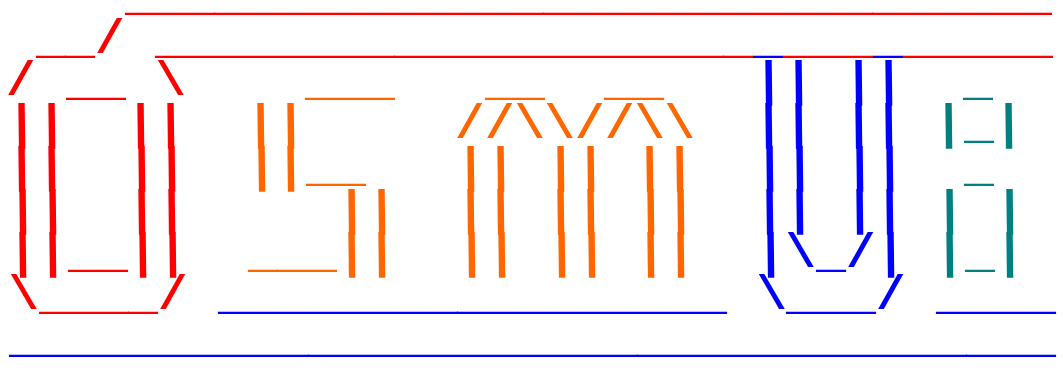
\includegraphics [width = 15cm ]{../projektplan/Logo_Osmui.png}  \\
Manual of OsmUi}

\begin{document}
\maketitle
\newpage
\tableofcontents
\newpage

\section {Notes}
\subsection {authors and website}
\subsection {readers}
This guide is intended for all users of OsmUi and those who want to be.
\subsection {Supported platforms}
OsmUi completely made out of Java code. Therefore, it runs on all Java SE compatible systems, eg Linux or Windows.


\section {} Download and Installation
\subsection {Installation and starting the program}
\subsubsection {Windows}
Open the file by klicking twice on OsmUi.exe.
\subsubsection {Linux, etc}
Proceed to the directory in which the OsmUi.jar fileis located via the console. Enter java-jar OsmUi.jar.

\section {Description of the program}
OsmUi is a user interface for the command line tool Osmosis. OsmUi translates the abstract concept of Osmosis' pipelines to a graphical representation which makes the entire functionality of Osmosis accessible, but is much more user friendly. While at Osmosis, a long command line call describes a pipeline for processing OpenStreetMap data, with OsmUi you should be able to "click together" a processing pipeline. Here, the functioning of the various tasks and the interactions can be seen on the user interface. 

\section {main screen}
After starting OsmUi always an empty file can be seen. You now have the option of either loading a file to load or export or create a new pipeline.

\section {Structure of the screen}
The largest part of the screen occupies the Pipelinebox. It is located right on the screen indicating the current Pielinen. Under it, the current pipeline as Osmosis call is displayed. Left, the Taskbox can be seen. It displays all currently insertable tasks. In its place you can also see the parameter box where the parameters of a task can be changed.

\section {Load and Save}
To save pipelines with all details such as position of shifted tasks, as well as non-executable pipelines OsmUi uses its own file format (. smu).
\subsection {Load File}
To load a saved pipeline choose \textbf {file} $ \rightarrow $ \textbf {store ...}. This opens a dialog box through which you can choose the path to the file. The charging process must now be confirmed. Only .smu files can be loaded.
\subsection {Save pipeline}
To save the current pipeline choose \textbf {file} $ \rightarrow $ \textbf {Save}. If the pipeline has already been saved once, the memory file is overwritten. Otherwise, the save-as menu is opened.
\subsection {Save pipeline}
To save the current pipeline choose \textbf {file} $ \rightarrow $ \textbf {Save ...}. This opens a dialog box where you can specify the location and name you want. After confirming a storage file is created.

\section {import and export}
To stay connected with other surfaces and already collected Osmosis calls, OsmUi offers various import and export functions. Only consistent pipelines can be exported.
\subsection {import pipeline from clipboard}
When importing from the clipboard the Osmosis call is read directly from the
Clipboard. For this you choose \textbf {file} $ \ rightarrow $ \textbf { Import from clipboard}.
\subsection {Import pipeline from file}
Here OsmUi reads an Osmosis call from a call script. There are both, .Bat
Files, as well .Sh files supported. For this you choose \textbf {file} $ \ rightarrow $ \textbf {Import from file}.
\subsection {export pipeline}
OsmUi can call pipeline as .sh format for all POSIX-compliant systems, as well as the .bat export format for Windows. The path with which Osmosis is called can be set here by the user. If these these includes a .jar file "java-jar "is hanged before. For this you choose \textbf {file} $ \ rightarrow $ \textbf{Export}.


\section {processing pipeline}
\subsection {create new pipeline}
To create a new pipeline, you select \textbf {file} $ \ rightarrow $ \textbf {New}. When a previously unsaved pipeline exists, you are asked whether it should be stored.
\subsection {add task}
\subsubsection {Input tasks}
To add a task without inputs you select in the Taskbox the desired input task and confirm with the button''Add''
\subsubsection {tasks with inputs}
To add a task first you need to select the task to which should be appended. This is done by a single click. Now in the Taskbox all compatible tasks are displayed. From these one can be attached, whith selecting and then click''Add''
\subsection {link tasks}
If two existing tasks should be connected, you move your mouse over the task until it is outlined in green. Next you left-click on the task and draw the resulting arrow on the task to be attached.
\subsection {Remove Task}
If a task should be removed, you must select it (single click) and press the delete key on the keyboard.
\subsection {change task parameters}
To change the parameters of a task you do a double-click on the appropriate task. Now all parameters are displayed in the left Parametertab. These can now be changed. In this case, all fields are required.
\subsection {remove link}
To remove the connection between two tasks, you must select it (single click). Then you press the delete key on the keyboard.

\section {copy Osmosis call}
The Osmosis call can be copied from the copy bar to, for example, integrate it into other documents. For this, you must highlight it and press Ctrl + C on your keyboard. The call can now be imported from the clipboard.

%\section {Tools}
%\subsection {Undo}
%If a change should be undone, choose \textbf {Edit} $ \ rightarrow $ \textbf {Undo}.
%\subsection {Recovering}
%If a reverse-made step should be restored just select \textbf {Edit} $ \ rightarrow $ \textbf {restore}.

\section {End Program}
To end OsmUi choose \textbf {file} $ \ rightarrow $ \textbf {end}.

\section {diff}
\begin {itemize}
\item 1.0 - Preparation of the Handbook (24/01/11)
\end {itemize}

\end {document} 